\documentclass{report}
\usepackage[utf8]{inputenc}
\usepackage[margin=1.8cm]{geometry}
\usepackage{fancyhdr}
\pagestyle{fancy}
\usepackage{graphicx}
\usepackage{titlepic}
\usepackage{indentfirst}
\usepackage[spanish]{babel}
\usepackage{csquotes}
\usepackage{array}
\usepackage{amsmath}
%\usepackage{longtable}
\usepackage{hyperref}
\usepackage{biblatex}
\usepackage{physics}
\usepackage{listings}
\usepackage{wrapfig}
\usepackage{pdflscape}
\addbibresource{Bibliografia.bib}

\hypersetup{
    colorlinks=true,
    linkcolor=cyan,
    urlcolor=black,
    linktoc=all,
}

\newcommand{\sizefont}{%
\fontsize{13}{16}\selectfont}
\renewcommand{\figurename}{Imagen}
\renewcommand*\contentsname{Indice}
\renewcommand{\arraystretch}{1.5}
\lstset{numbers=left, numberstyle=\tiny, numbersep=5pt}

\font\myfont=cmr12 at 25 pt
\title{\myfont Proyecto 2.\\Algoritmos paralelos: Transformada de Fourier
}
\titlepic{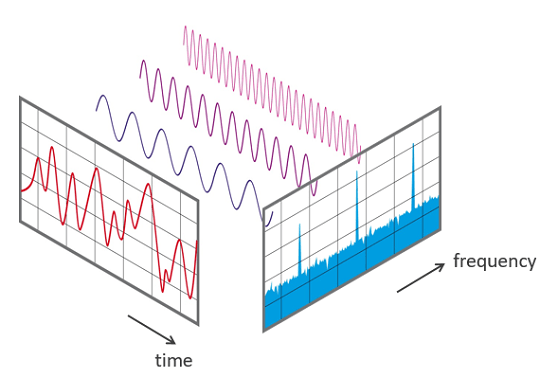
\includegraphics[width=\textwidth]{Images/Portada.png}}
\author{David, Calderón Jiménez
        \\ Humberto Ignacio, Hernández Olvera
        \\ Iñaky, Ordiales Caballero}
        
\date{17/Enero/2021}

\begin{document}
\begin{titlepage}
    \begin{center}
        \vspace*{1 cm}
        
        \Huge
        \textbf{\myfont Proyecto 2}
        
        \vspace{0.5cm}
        Algoritmos paralelos: Transformada de Fourier.
        
        \vspace{1.5cm}
        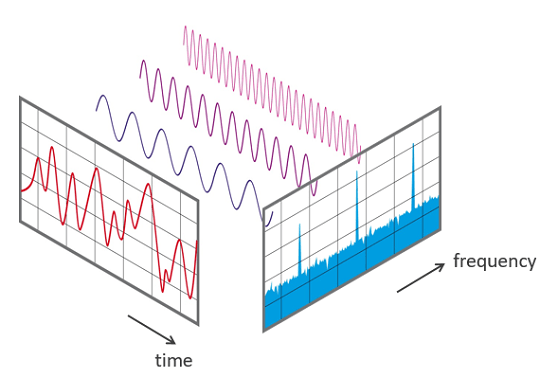
\includegraphics[width=0.9\textwidth]{Images/Portada.png}
        
        \vspace{2cm}
        \LARGE 
        \textbf{Equipo 4\\}
        
        \vspace{0.3cm}
        \Large 
        Calderón Jiménez, David\\
        Hernández Olvera, Humberto Ignacio\\
        Ordiales Caballero, Iñaky
        
        \vspace{0.5cm}
        20 de Enero del 2021.
        \vspace{3cm}
    \end{center}
\end{titlepage}
\fancyhf{}
\fancyfoot[R]{\sizefont Página \thepage}

\section*{Descripción General del Proyecto}
\noindent Para este segundo proyecto se deberá realizar un \underline{trabajo de investigación} acerca de algún algoritmo, alguna arquitectura o alguna forma de implementación de la programación paralela. Así mismo, se deberá realizar un video para la presentación de los puntos mas relevantes del trabajo de investigación.

\section*{Objetivo}
\noindent
Que el alumno ponga en práctica los conceptos de la programación paralela a través de la implementación de un algoritmo paralelo, así mismo desarrolle su capacidad para responder
preguntas acerca de un concepto analizado a profundidad.
\subsection*{Objetivos personales}
\noindent
Nuestro objetivo como equipo para este proyecto es lograr un gran entendimiento del algoritmo empleado para calcular computacionalmente la transformada de Fourier. Y de este modo poder explicar de forma clara y precisa su implementación y funcionamiento desde una perspectiva paralela.

\section*{Introducción}

\noindent 
A lo largo del curso de EDA 2 hemos estudiado diversos temas sobre las estructuras de datos y los algoritmos. El último tema que se encuentra en el temario es la \textit{Introducción a los Algoritmos Paralelos}. En la clase de teoría, así como en las prácticas del laboratorio hemos podido aprender los conceptos básicos de la programación paralela, así como hemos desarrollado programas simples que la usen. Sin embargo, hasta ahora no hemos revisado un uso e implementación de la vida real de este tipo de algoritmos. En este trabajo se explorará el algoritmo \textbf{\textit{Fast Fourier Transform} (FFT)} o transformada rápida de Fourier. Pero antes de poder llegar al paralelismo del algoritmo, primero se requieren explicar otros temas.\medskip

Uno de los aspectos de mayor importancia dentro de la programación es la eficiencia de los algoritmos/programas. Existen diferentes formas de medir la eficiencia de un programa o un procesador, ya sea por espacio de memoria o por tiempo. Viéndolo desde el punto de vista del tiempo la eficiencia depende directamente de cuánto se tarda en ejecutar una instrucción básica y del número de instrucciones básicas que pueden ser ejecutadas concurrentemente. Esta eficiencia puede ser incrementada por avances en la arquitectura como el aumento del tamaño de la palabra del procesador (8, 16, 32, 64 bits) y por avances tecnológicos en transistores y demás componentes electrónicos. El avance en la arquitectura mediante el tamaño de palabra del procesador incrementan la cantidad de trabajo que se puede realizar por ciclo de instrucción. Con los 32 o 64 bits de las computadora modernas realmente ya no se obtiene mucho beneficio de seguirlas aumentando. Al menos por el momento se encuentran en su estado más optimo. Por el otro lado, tenemos los componentes electrónicos. Al mejorar estos, se disminuye el tiempo del ciclo del procesador, es decir el tiempo para ejecutar la operación más básica. Sin embargo, actualmente estos tiempos ya decrecen muy poco con cada mejora y parece que están alcanzando límites físicos como la velocidad de la luz. Esto significa que pronto tampoco se podrá mejorar el tiempo de ejecución mejorando los componentes electrónicos. Esto nos lleva a la pregunta, ¿Cómo podemos seguir eficientizando la programación? \medskip

Al no poder depender de procesadores más rápidos para obtener más eficiencia, la solución es un cambio de paradigma en la programación. Más en específico el usar la \textbf{Programación Paralela}. La programación paralela parte de la idea del multiprocesamiento. El multiprocesamiento es el usar más de un procesador a la vez (o por lo menos varios núcleos) para realizar en conjunto una serie de instrucciones. Entonces un programa paralelo es aquel formado por varios procesos que se ejecutan en múltiples procesadores conectados entre sí mediante una red de comunicación. Todo esto siguiendo un esquema de paralelismo espacial, el cual se expresa físicamente en varios procesadores operando en simultáneo. Los beneficios que se obtienen con este paradigma es el lograr en muchas ocasiones disminuir los tiempos de ejecución y volver más eficientes los programas. Sin embargo, el paralelismo no siempre es posible, y aún cuando sí lo es, puede no volver más eficiente el programa debido a los tiempos de comunicación entre los procesadores. Todo esto se tiene que estudiar al momento de querer paralelizar algún algoritmo ya existente, o al tratar de crear uno desde cero. En este trabajo se estudia la paralelización del algoritmo ya existente de la transformada rápida de Fourier. Se revisará el algoritmo, su implementación y sus medidas de eficiencia.\medskip

\clearpage
\section*{Transformada de Fourier}
\noindent Antes de llegar a ver los algoritmos, primero hay que entender aunque sea superficialmente la trasformada de Fourier. Una transformada es un operador especial matemático que representa una transformación entre dos bases diferentes. Dentro de las transformaciones existen un subconjunto llamado transformaciones integrales, éstas son una función (la cual se centra en el cálculo de una integral) que se aplica sobre alguna otra función para llevarla de un dominio a su expresión equivalente en otro dominio. La transformada de Fourier, es una caso especial de una transformación integral. Denominada así por Joseph Fourier, se emplea comúnmente para llevar funciones o señales desde el dominio del tiempo (o espacial) hasta el dominio de la frecuencia. A pesar de que en un inicio esto tal vez no nos parezca tan relevante, la Transformada de Fourier es una de las más importantes (puede que sea la más importante) que se hayan descubierto en las matemáticas. Algunos de los usos más importantes en la matemática, física e ingeniería los vemos en el procesamiento de señales (electrónicas), comunicaciones, óptica, procesamiento de imágenes y medicina, por mencionar algunos.\medskip 
\begin{wrapfigure}{l}{0.25\textwidth}
        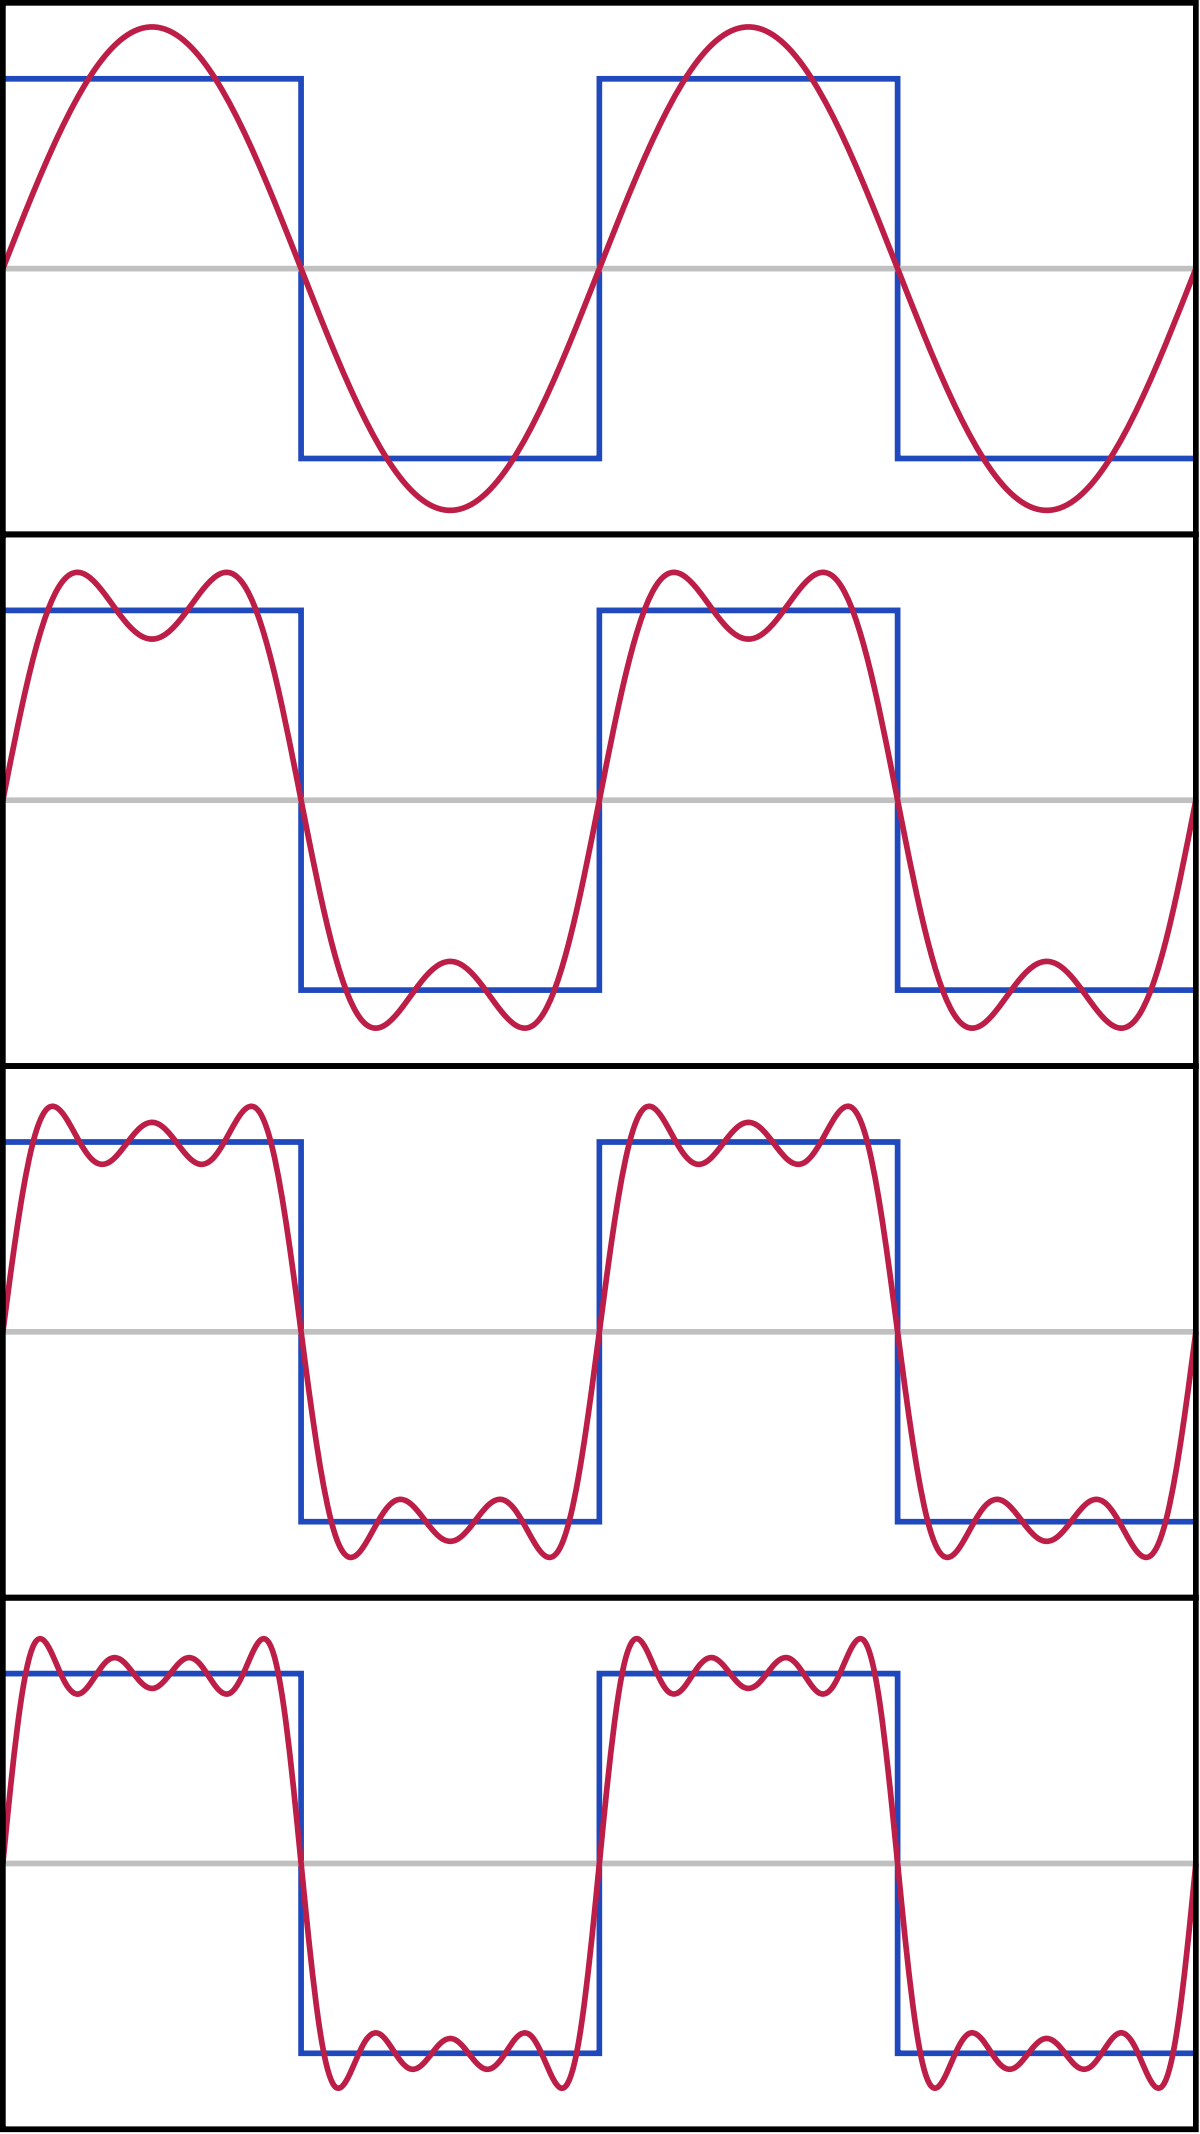
\includegraphics[scale=0.1]{Images/fourier2.png}
        \caption{Diagrama de FFT}
\end{wrapfigure}

El que nos ha interesado más desde el punto de vista ingenieril es el de procesamiento de señales electrónicas, ya que esta aplicación fue lo que nos permitió evolucionar de gran forma las telecomunicaciones. Los ejemplos iniciales más grandes del uso de la transformada de Fourier están en la radio, donde a través de ella podemos filtrar las diferentes frecuencias y concentrarnos en sólo una. Pero además de eso la utilizamos en las redes como el wi-fi, el internet, o la telefonía móvil. Éstas no existirían como los conocemos hoy en día si nos fuera por la transformada de Fourier. Fue gracias a su gran cantidad y relevancia de usos que se vio casi natural el computalizar sus cálculos para facilitar su obtención. Esto ya que para cada señal, la transformada es una operación diferente y a pesar de tener tablas que facilitan el cálculo, en muchas ocasiones no es sencillo realizarlo. Por eso se planteó en un inicio un algoritmo secuencial que pudiera realizarla. Pero para poder ver bien el algoritmo antes repasemos qué es y de dónde sale la idea de una Transformada de Fourier.\medskip

La transformada de Fourier surge de las series de Fourier. A su vez la serie de Fourier surge de la idea que cualquier función periódica puede ser representada mediante una suma infinita de senos y cosenos. Existen dos tipos de series de Fourier. La trigonométrica y la compleja. La trigonométrica es un termino constante más una suma infinita de funciones coseno más una suma infinita de funciones seno. La serie trigonométrica de Fourier se define para una función $f\left( t\right) $ en un intervalo $-L<x<L$ donde la función es periódica de la siguiente manera:

\[
f\left( t\right) =\frac{a\left( 0\right) }2+\sum\limits_{n=1}^\infty \left[
a\left( n\right) \cos \frac{n\pi t}L+b\left( n\right) \sin \frac{n\pi t}%
L\right] 
\]

\noindent donde $a\left( 0\right) $, $a\left( n\right) $ y $b\left( n\right) $ son los coeficiente de Fourier definidos como:

\begin{eqnarray*}
a\left( 0\right) &=&\frac 1L\int_{-L}^Lf\left( t\right) dx \\
a\left( n\right) &=&\frac 1L\int_{-L}^Lf\left( t\right) \cos \frac{n\pi t}Ldx
\\
b\left( n\right) &=&\frac 1L\int_{-L}^Lf\left( t\right) \sin \frac{n\pi t}Ldx
\end{eqnarray*}

\noindent A su vez de la serie trigonométrica se puede llegar a la serie compleja. La serie compleja de Fourier parte de que el periodo de una función $f\left( t\right) $ es $T$ y $C_n$, $w_0$ son:

\[
w\left( 0\right) =\frac{2\pi}{T}
\]

\[
C\left( n\right) = \frac{a_n - ib_n}{2} =\frac{1}{T}\int\limits_{\frac{-T}{2}}^{\frac{T}{2}} f\left( t\right) e^{-inw_0t} dt
\]

\noindent Así la serie compleja de Fourier es:

\[
f\left( t\right) =\sum\limits_{n=1}^\infty \left[
C\left( n\right) e^{inw_{0}t}\right] +\sum\limits_{n=-1}^{-\infty} \left[C\left( n\right) e^{inw_{0}t}\right] 
\]

\[
f\left( t\right) =\sum\limits_{n=-\infty}^\infty \left[
C\left( n\right) e^{inw_{0}t}\right] 
\]

Una vez se tiene la serie compleja de Fourier y bajo la idea de que cualquier función es periódica en el intervalo $(\infty, -\infty)$ mediante algunos cálculos que no se muestran en este documento llegamos a la dichosa \textbf{Transformada de Fourier} y a su vez a la transformada inversa. El propio término se refiere tanto a la operación de transformación como a la función que produce.\medskip

\begin{figure}[h!]
    \centering
    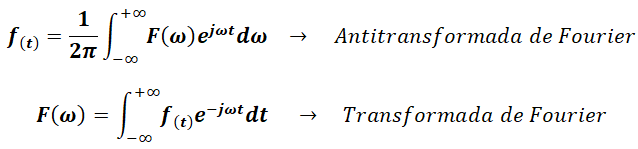
\includegraphics[scale=0.6]{Images/Fourier.png}
    \caption{Transformada de Fourier.}
    \label{Fourier}
\end{figure}

Sin embargo la computalización de esta transformada no sea hace directamente, ya que sería un proceso laborioso y costoso computacionalmente hablando. Para mejorar esto se creó la Transformada Discreta de Fourier, de la cual deriva la versión ya programable, la Transformada Rápida de Fourier. En las siguientes secciones se hablará más de esto.

\section*{Algoritmo Secuencial Transformada de Fourier}
\noindent La transformada rápida de Fourier, conocida por la abreviatura FFT (del inglés Fast Fourier Transform) es un algoritmo eficiente que permite calcular la transformada de Fourier discreta (DFT) y su inversa. La FFT es en ocasiones catalogado como el algoritmo más poderoso del último siglo. Esto debido a su de gran importancia en una amplia variedad de aplicaciones, desde el tratamiento y filtrado digital de señales, compresión de imágenes y audio, resolución de ecuaciones diferenciales parciales o inclusive en los algoritmos de multiplicación rápida de grandes enteros. Para poder presentar el algoritmo, lo único que nos falta es ver la transformada discreta de Fourier (que en realidad es una serie) y porqué se usa ésta.\medskip
\begin{wrapfigure}{r}{0.3\textwidth}
\begin{center}
    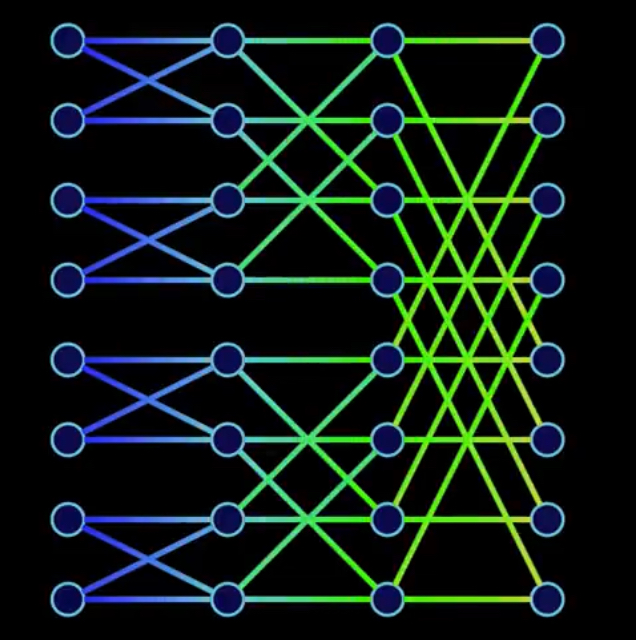
\includegraphics[scale=0.24]{Images/FFT circuit.jpg}
    \caption{Circuito del cómputo de la transformada de Fourier}
\end{center}
\end{wrapfigure}

\subsection*{Discrete Fourier Transform (DFT)}
En la mayoría de los casos no se cuenta con funciones analíticas desde las cuales se puede calcular una transformación continua, sino que se tienen mediciones experimentales o mediciones de simulaciones. Por esto en realidad lo que se tiene son $N$ medidas puntuales en un intervalo de $[x_0, x_n]$. Por lo que tenemos un vector de datos $[x_0, x_1, x_2, ..., x_n]^T$ con los que queremos obtener la serie de Fourier para cada uno de esos puntos. Y esto es lo que hace la Transformada de Fourier. A continuación se defina la Transformada Discreta de Fourier:

\[
\hat{x}_k = \sum\limits_{n=0}^{N-1} \left[ x_ne^{\frac{-i2\pi}{N}kn}\right]
\]
La Transformada Discreta Inversa de Fourier es:

\[
x_n = \sum\limits_{n=0}^{N-1} \left[ \hat{x}_ne^{\frac{i2\pi}{N}kn}\right]
\]

\noindent donde $\hat{x}_k$ es el k-ésimo coeficiente de Fourier y $x_n$ es el n-ésimo dato del intervalo.

\subsection*{Fast Fourier Transform (FFT)}
\noindent Ahora bien, la Transformada Discreta de Fourier es una transformación matemática que puede ser escrita en términos de una multiplicación de matrices muy grandes. La Transformada Rápida de Fourier es una forma computacionalmente eficiente de calcular la transformada discreta para conjuntos de datos muy grandes. En cierto modo son sinónimos, FFT es cómo computamos la DFT.
Cuando se habla del tratamiento digital de señales, el algoritmo FFT impone algunas limitaciones en la señal y en el espectro resultante ya que la señal muestreada y que se va a transformar debe consistir de un número de muestras igual a una potencia de dos.\medskip

El algoritmo secuencial de la Fast Fourier Transfrom se basa en el principio de "divide y vencerás". Aprovecha la periodicidad de los datos (siendo el periodo $T = x_n - x_0$) y de la simetría de la transformada al trabajar con conjugados complejos.La transformada discreta de Fourier puede ser reescrita en forma matricial de la siguiente forma:\medskip

\begin{gather}
    \begin{bmatrix}
        \hat{x}_0 \\ \hat{x}_1 \\ \hat{x}_2 \\ ... \\\hat{x}_n
    \end{bmatrix}
    =
    \underbrace{
    \begin{bmatrix}
        1 & 1 & 1 & ... & 1\\
        1 & w_n & w_n^2 & ... & w_n^{n-1}\\
        1 & w_n^2 & w_n^4 & ... & w_n^{2(n-1)}\\
        . & . & . & . & .\\
        1 & w_n^{n-1} & w_n^{2(n-1)} & ... & w_n^{(n-1)^2}\\
    \end{bmatrix}
    }_{Matriz\:de\:Transformacion\:Directa\:de\:Fourier\:\textbf{DFT}}
    \begin{bmatrix}
        x_0 \\ x_1 \\ x_2 \\ ... \\ x_n
    \end{bmatrix}
\end{gather}

\noindent
Esta puede ser simplificada de la siguiente forma (múltiples veces):

\begin{gather}
    \begin{bmatrix}
        \hat{x}_0 \\ \hat{x}_1 \\ \hat{x}_2 \\ ... \\\hat{x}_n
    \end{bmatrix}
    =
    \begin{bmatrix}
        [I_{\frac{n}{2}\times\frac{n}{2}}] & -[D_{\frac{n}{2}\times\frac{n}{2}}]\\
        [I_{\frac{n}{2}\times\frac{n}{2}}] & -[D_{\frac{n}{2}\times\frac{n}{2}}]
    \end{bmatrix}
    \begin{bmatrix}
        [DFT_{\frac{n}{2}\times\frac{n}{2}}] & 0\\
        0 & [DFT_{\frac{n}{2}\times\frac{n}{2}}]
    \end{bmatrix}
    \begin{bmatrix}
        [x_{par}] \\ [x_{impar}]
    \end{bmatrix}
\end{gather}

\vspace{0.7cm}

\noindent
\large 
La idea general del algoritmo es la siguiente:\medskip
\noindent
\textbf{Inicio.}
\begin{enumerate}
    \item Dividir el vector de datos inicial en dos vectores, uno para los índices par y otro de los índices impar. (pasar de la ecuación 1 a la ecuación 2).
    \item Obtener las matrices diagonales y sub-matrices de transformación correspondientes.
    \item Se puede repetir el paso 1 y 2 las veces que sea deseado. Estas serán las etapas de descomposición.
    \item Realizar la multiplicación de matrices resultante.
    
\end{enumerate}
\textbf{Fin.}

\vspace{0.2cm}

\normalsize
\noindent El algoritmo se puede ver de manera gráfica en el diagrama de la figura 4 en la siguiente página.\medskip

Algo interesante de notar es que antes de ser paralelizado, el algoritmo FFT ya es bastante más eficiente que implementar directamente la transformada discreta. FFT tiene una complejidad temporal de $O(n\log n)$ mientras que DFT tiene una complejidad temporal de $O(n^2)$, por lo que ya representa una mejora con tan solo usar el algoritmo FFT que realiza una multiplicación de matrices en lugar de varios ciclos for anidados.\medskip

\vfill

\noindent
\textit{\textbf{***} Como dato curioso, se ha encontrado que el matemático alemán Carl Friedrich Gauss, apodado el "príncipe de las matemáticas, desarrolló y usó un algoritmo muy parecido al FFT moderno en 1805. Inclusive siendo esta fecha anterior a la publicación de los estudios harmónicos de Fourier (1807).}

\begin{figure}[h!]
    \begin{center}
        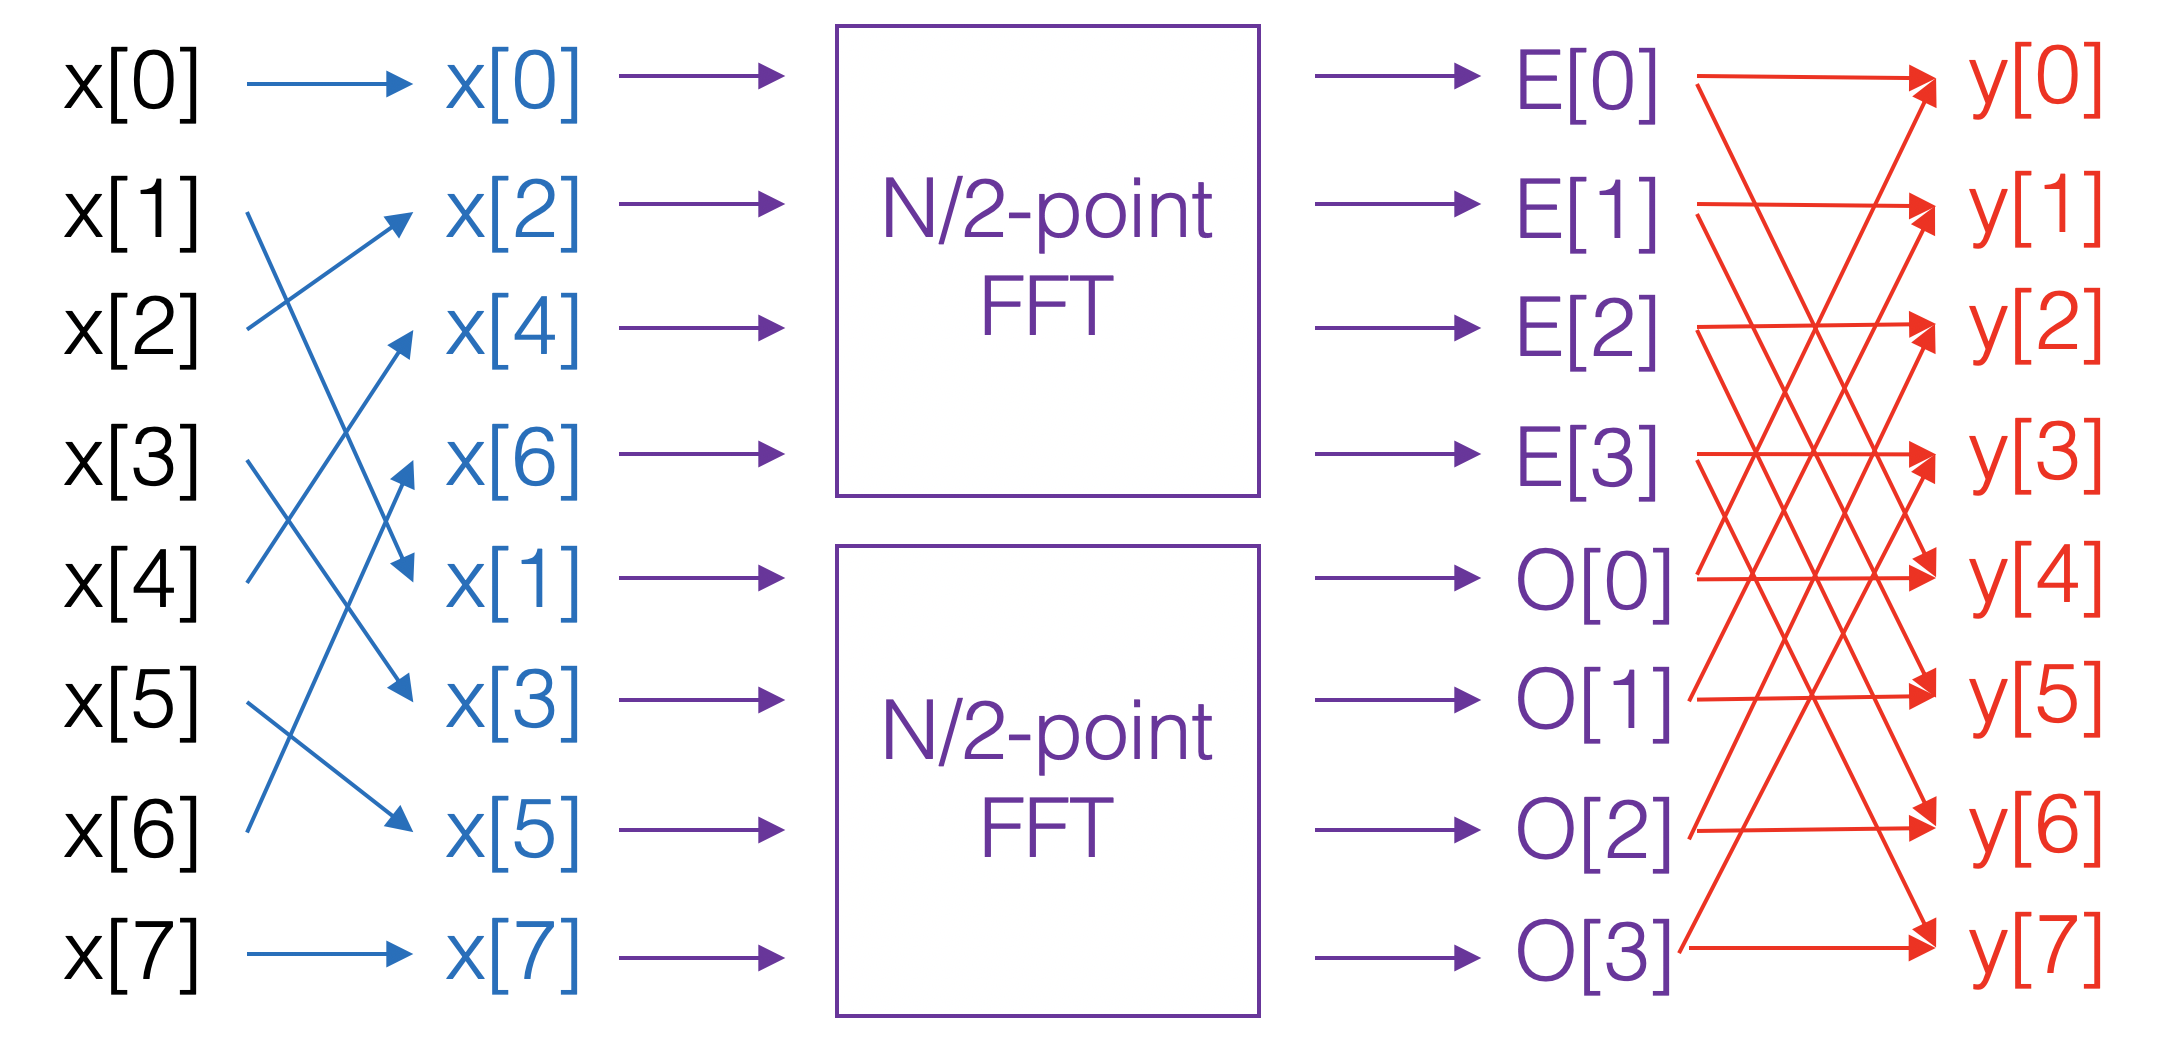
\includegraphics[width=\textwidth]{Images/fft_diagram.png}
        \caption{Diagrama de FFT}
    \end{center}
\end{figure}

\clearpage

\section*{Paralelización}
\noindent La Transformada Discreta de Fourier (DFT) es un problema para el cual hay una larga historia de algoritmos paralelos. El algoritmos para la Transformada Rápida de Fourier (FFT) para resolver la DFT es sencillo de paralelizar. Proporciona dos oportunidades principales de paralelización, siendo uno las sub divisiones de los vectores de datos y el otro la multiplicación de matrices. Además de éstas dos áreas, gran parte de la investigación se ha ido en reducir los costos de comunicación siendo una parte vital y complicada de la programación paralela. La topología que se ha encontrado más eficiente es la de red de mariposa. Y el algoritmo FFT es tan importante que la topología de red de mariposa es también llamada red FFT ya que es dónde más común se ve esta topología.

\subsection*{Algoritmo en paralelo}
El algoritmo paralelo para la transformada de Fourier rápida es sencillo de entender una vez se comprende el algoritmo secuencial. A continuación se muestra un ejemplo de algoritmo FFT paralelo sobre números complejos:
\vspace{0.4cm}

\noindent
\textbf{\large FFT(A)}\medskip

\begin{lstlisting}[frame=single, mathescape]
n = |A|
if (n=1) then return A
else
    in parallel do
        EVEN = FFT({A[2i : i $\in$ [0..n/2]})
        ODD = FFT({A[2i + 1] : i \in [0..n/2] })
    return {EVEN[j]+ODD[j]$e^{2\pi ij/n}$:j$\in$[0..n/2]}++{EVEN[j]-ODD[j]$e^{2\pi ij/n}$:j$\in$[0..n/2]}

\end{lstlisting}

Simplificando su funcionamiento, el algoritmo se llama recursivamente en los elementos \textit{odd} y \textit{even} y después junta los resultados. El algoritmo tiene una complejidad temporal de O\textit{(n} log \textit{n)}, así como su versión secuencial, y tiene una profundidad recursiva de O\textit{(}log \textit{n)}. Lo importante de notar aquí (quedará más claro al revisar la topología) es que la paralelización se lleva a cabo conjunto con la recursividad.\medskip

\subsection*{Topología de red de mariposa}

\noindent La topología de red de mariposa es una técnica para enlazar múltiples computadoras a una red de alta velocidad. Esta forma de topología de red de interconexión multi-etapa puede ser usada para conectar diferentes nodos en un sistema multiprocesador. En el algoritmo FFT se usa esta topología donde cada nodo es una unidad de procesamiento que podrá trabajar con una fracción de los datos iniciales. Pero como vimos en el algoritmo, la comunicación es muy importante, ya que para calcular los coeficientes de fourier se usa un dato par y uno impar del vector inicial. Debido a esto se necesita esta topología que tiene exactamente los canales de comunicación entre procesadores necesarios.\medskip

\begin{figure}[h!]
    \centering
    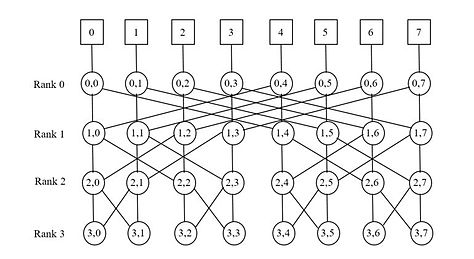
\includegraphics[scale=1.4]{Images/Butterfly_Network.jpg}
    \caption{Topología de red de mariposa.}
    \label{Topologia mariposa}
\end{figure}

\clearpage
\subsection*{Tipo de paralelismo}
\noindent El tipo de paralelismo que se utiliza en este algoritmo es el de \textbf{paralelismo de datos}.Éste es un paradigma de la programación concurrente que consiste en subdividir el conjunto de datos de entrada a un programa, de manera que a cada procesador le corresponda un subconjunto de esos datos. Cada procesador efectuará la misma secuencia de operaciones que los otros procesadores sobre su subconjunto de datos asignado. En resumen: se distribuyen los datos y se replican las tareas. Idealmente, esta ejecución simultánea de operaciones, resulta en una \textbf{\textit{aceleración neta global del cómputo}}.\medskip

Para este ejemplo en particular del algoritmo rápido de la transformada de Fourier utilizaremos este tipo de paralelismo, pues este es es el mas adecuado gracias a que la mayor parte del programa depende de ciclos, los cuales al paralelizarlos cada procesador efectúa la misma operación pero con diferentes datos asignados. 

\subsection*{Métricas de desempeño}
Para una N igual 1, vemos que el algoritmo secuencial se ejecuta en menos tiempo que su versión paralela.\medskip

Para una N igual a 10, el algoritmo secuencial es ahora más lento que su versión paralela, y mientras se siga incrementando el valor de N, la versión paralela sigue siendo más rápida que la secuencial.\medskip

\noindent \textbf{\textit{Todos los datos usados en las siguientes gráficas son el promedio de 5 ejecuciones para cada situación particular.}}

\subsection*{Comparativa de Tiempos}
\noindent Las siguiente gráfica es una comparativa del tiempo que se tarda el programa en calcular la transformada de Fourier para una medida experimental de 150 puntos. (Idealmente en la vida real estos serían alguna señal digital captada que se está tratando de filtrar).

\vspace{0.7cm}

\begin{figure}[h!]
    \centering
    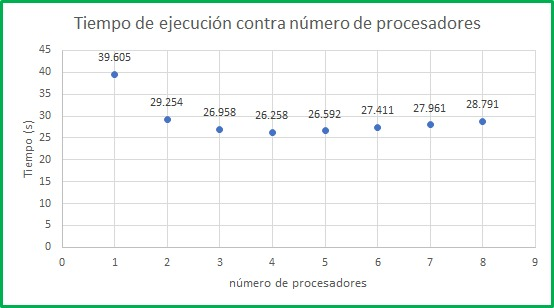
\includegraphics[width = 0.75\textwidth]{Images/tiempo.jpeg}
    \caption{Gráfica 1. Comparativa de Tiempos}
\end{figure}

En la gráfica podemos observar como el tiempo con un sólo procesador, es decir al realizar una ejecución totalmente secuencial se tarda 39.605 segundos en calcular los 150 coeficientes de Fourier necesarios. De ahí conforma vamos agregando más unidades de procesamiento el tiempo va bajando, hasta llegar a un óptimo con respecto del tiempo en 4 procesadores. Después para 5, 6, 7, 8 procesadores se empieza a tardar más tiempo. Aunque nunca llega cercano a los 39.605 del procesamiento único.

\clearpage
\subsection*{Speedup}
\noindent El Speedup es la relación de tiempo de ejecución de un programa ejecutándose en un solo procesador sobre el tiempo de ejecución del mismo programa ejecutándose en \textit{n} procesadores. Esta medida es muy parecida con respecto a la gráfica anterior (del tiempo neto). Sin embargo ahora se mide qué tan más rápido es el uso de múltiples procesadores con respecto a uno sólo. Esta métrica solo considera aspectos temporales, no toma en cuenta otros como la topología elegida, el balance de carga, la granularidad, etc.\medskip
\begin{equation*}
    S(n) = \frac{T(1)}{T(n)}
\end{equation*}

\vspace{0.5cm}

\begin{center}
    \begin{tabular}{|c|c|c|c|c|c|c|c|c|}
        \hline
           Num. Procesadores & 1 & 2 & 3 & 4 & 5 & 6 & 7 & 8 \\
        \hline
            Speedup & 1.0 & 1.35 & 1.47 & 1.51 & 1.49 & 1.45 & 1.42 & 1.38 \\
        \hline
    \end{tabular}
\end{center}

\vspace{0.5cm}

\begin{figure}[h!]
    \centering
    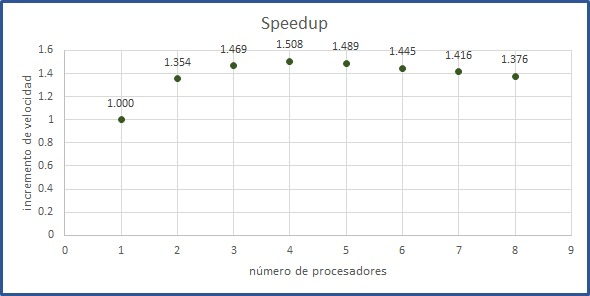
\includegraphics[width = 0.75\textwidth]{Images/Speedup.jpeg}
    \caption{Gráfica 2. Speedup}
\end{figure}

\vspace{0.2cm}

En la gráfica de arriba podemos ver como la medida de Speedup parte de que el tiempo que tarda en un sólo procesador será la medida de una unidad de velocidad. Los demás datos son cuántas veces se incrementa la velocidad con n número de procesadores. Al igual que con la gráfica temporal (son los mismo datos expresados diferentes), vemos que el punto más óptimo es con cuatro procesadores. Al usar los cuatro procesadores en paralelo se tiene 1.508 veces la velocidad de ejecución inicial. Después para 5, 6, 7, y 8 empieza a bajar esta cantidad. Las razones más probables de esto, son que para la cantidad de datos usadas (150 medidas) la subdivisión de cálculos es eficiente entre cuatro, pero después los tiempos de comunicación entre los procesadores es mayor al beneficio de seguir dividiendo las tareas. Esto podría cambiar si se usaran más o menos datos.

\clearpage
\subsection*{Eficiencia}
\noindent Se asocia a la idea de que \textit{n} procesadores deben hacer el trabajo en una fracción \textit{$\frac{1}{n}$} del tiempo que le lleva a un solo procesador. Esta medida toma en cuenta el porcentaje de aprovechamiento de cada procesador individual que se use.\medskip
\begin{equation*}
    E(n) = \frac{T(1)}{n \cdot T(n)} = \frac{S(n)}{n}
\end{equation*}

\vspace{0.5cm}

\begin{center}
    \begin{tabular}{|c|c|c|c|c|c|c|c|c|}
        \hline
           Num. Procesadores & 1 & 2 & 3 & 4 & 5 & 6 & 7 & 8 \\
        \hline
            Eficiencia & 1.0 & 0.67 & 0.49 & 0.38 & 0.30 & 0.24 & 0.20 & 0.17 \\
        \hline
    \end{tabular}
\end{center}

\vspace{0.5cm}

\begin{figure}[h!]
    \centering
    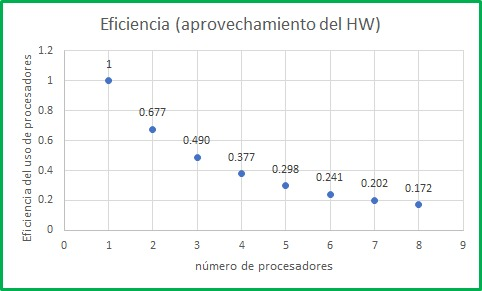
\includegraphics[width = 0.75\textwidth]{Images/Eficiencia.jpeg}
    \caption{Gráfica 3. Eficiencia}
\end{figure}

\vspace{0.2cm}

El valor de la eficiencia refleja el aprovechamiento de los recursos de Hardware del sistema, por lo tanto, siempre será menor a 1. Se parte nuevamente de la idea que el aprovechamiento máximo del procesador es realizar la ejecución en 39.605 segundos que es lo que tardó un sólo procesador en hacerlo. Entonces para seguir teniendo un aprovechamiento del 100\% ó 1 se tendría que realizar en dos procesadores en 19.802 segundos (la mitad). Esto desde la teoría no sería posible debido a que algo de tiempo se debe perder en la comunicación entre procesadores. En la gráfica vemos como donde más se aprovechan los recursos del procesador son con 2 procesadores. A partir de ahí todo va bajando. Esto es de esperarse, y da una perspectiva a las gráficas anteriores dónde podríamos creer que lo más óptimo era usar 4 procesadores. Pues aquí vemos que no se aprovechan arriba del 40\% cada uno de ellos.\medskip

\clearpage
\subsection*{Fracción Serial}
\noindent También conocida como métrica Karp-Flatt, relaciona el  Speedup y la eficiencia con el propósito de tomar en cuenta otros factores además del tiempo. Hay quienes piensan que la fracción serial proporciona un método más real de medir el rendimiento del proceso paralelo. La fracción serial determinada experimentalmente es una métrica muy útil por dos razones: primero toma en cuenta el costo de comunicación en procesos paralelos y segundo puede ayudar a detectar otras fuentes de retrasos o ineficiencias que son ignorados con los modelos temporales más simples. \medskip

\begin{equation*}
    \scalebox{1.5}{$f = \frac{\frac{1}{s} - \frac{1}{n}}{1-\frac{1}{n}}$}
\end{equation*}

\vspace{0.2cm}

\begin{center}
    \begin{tabular}{|c|c|c|c|c|c|c|c|}
        \hline
           Num. Procesadores  & 2 & 3 & 4 & 5 & 6 & 7 & 8 \\
        \hline
            f & 0.48 & 0.52 & 0.55 & 0.59 & 0.68 & 0.66 & 0.69 \\
        \hline
    \end{tabular}
\end{center}

\vspace{0.3cm}

\begin{figure}[h!]
    \centering
    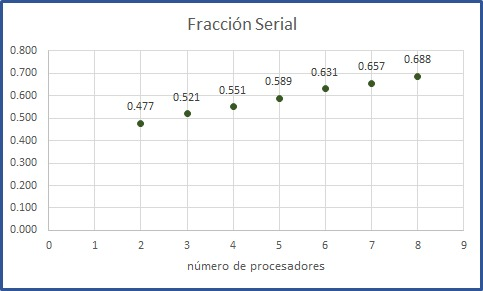
\includegraphics[width = 0.75\textwidth]{Images/fraccionSerial.jpeg}
    \caption{Gráfica 4. Fracción Serial}
\end{figure}

\vspace{0.2cm}

En esta última métrica que se analizó lo que podemos ver es qué tan paralelizadamente eficiente es el proceso. Nos permite distinguir si los decrementos en la eficiencia al aumentar en procesadores son debido a oportunidades limitadas de paralelizar o incrementos en la carga arquitectónica (mal balance de carga). Entre menor el valor de $f$ mejor la paralelización. Por esto podemos algo interesante que no habíamos visto en las otras métricas, y es que entre más procesadores, la fracción serial aumenta, en ningún lado hay un aparente punto de inflexión. Esto probablemente se debe a la cantidad limitada de datos con los que se trabajó. De haber usado más, probablemente veríamos un cambio en la monotonía de la gráfica. Según esta métrica en términos de paralelización lo mejor es dos procesadores.

\vfill{}
\noindent \textbf{Habiendo visto estas métricas del paralelismo, queda la pregunta ¿Cuántos procesadores puedo usar para que mi ejecución sea lo más eficiente posible? La respuesta es que va depender de tus necesidades, tus capacidades (en términos de Hardware) y un poco de criterio personal. No se puede cumplir con todas las métricas de la manera más eficiente posible, se tendrán que aceptar niveles bajos en una para tener altos en otra. Por ejemplo si se cuenta con una capacidad grande de procesadores sin usarse y quieres el tiempo más rápido, podrías usar el punto más alto del Speedup aunque se desaprovechen los procesadores. O en caso de que se tengan muchos programas o la vez podrías buscar el mayor aprovechamiento de procesadores para usarlos en diferentes tareas. Así es que las métricas nos dan una idea del funcionamiento, pero finalmente la configuración debe ser decisión del programador.}
\clearpage


\subsection*{Formas de comunicación}

El medio de comunicación es por medio de la  memoria compartida, que es aquel tipo de memoria que puede ser accedida por múltiples programas, ya sea para comunicarse entre ellos o para evitar copias redundantes. La memoria compartida es un modo eficaz de pasar datos entre aplicaciones. Dependiendo del contexto, los programas pueden ejecutarse en un mismo procesador o en procesadores separados.

\begin{figure}[h!]
    \centering
    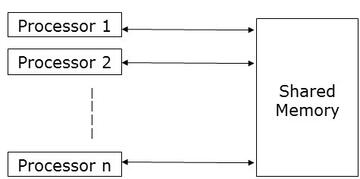
\includegraphics[width=0.6\textwidth]{Images/Memoria compartida.jpg}
    \caption{Diagrama Memoria compartida}
\end{figure}


\subsection*{Granularidad}

A partir de una comunicación por memoria compartida, podemos decir que la granularidad es de tipo fina pues la mayor parte del código se basa en las operaciones con matrices las cuales al trabajar con paralelismo de datos por lo cual al ser la mayor carga de trabajo en operaciones paralelas la granularidad se vuelve fina gracias a que el numero de llamadas es mayor , esto lo podemos comprobar en las pruebas que veremos a continuación, en donde al trabajar con pocos datos el numero de llamadas es mayor al de operaciones por lo que su versión secuencial es mas eficiente que la paralela cuando se trabaja con pocos datos.


\begin{figure}[h!]
    \centering
    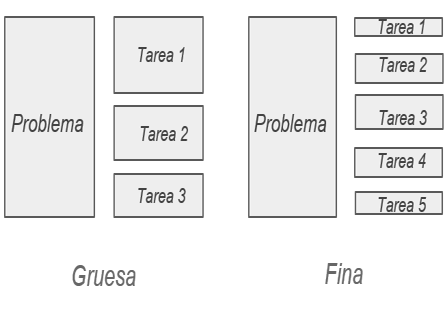
\includegraphics[width=0.6\textwidth]{Images/Granularidad.png}
    \caption{Tipos de Granularidad}
\end{figure}

\clearpage


\section*{Implementación} % CREO QUE FALTA ALGO 
El código seleccionado para llevar a cabo la Transformada Rápida de Fourier (FFT) se lleva a cabo utilizando el lenguaje C y la API OpenMP, este código no es de nuestra autoría \cite{FFT}, pero se modificó para que se pudiera adaptar a nuestras necesidades y poder reutilizarlo para las pruebas en su forma secuencial. Involucra las siguientes etapas, dentro de un ciclo for que se repite 20 veces:\medskip


\begin{enumerate}
    \item Se generan dos vectores de números complejos con números pseudo-aleatorios, almacenados en 4 arreglos, 2 contienen las partes reales de cada vector, y los otros 2 contienen las partes imaginarias de cada vector.
    \item Se inicializan las tablas de senos y cosenos que son necesarias para el cálculo de la FFT de acuerdo al valor de n.
    \item Se realiza un paso de la FFT hacia adelante y hacia atrás.
    \item Se repite el ciclo.
\end{enumerate}

\begin{figure}[h!]
    \centering
    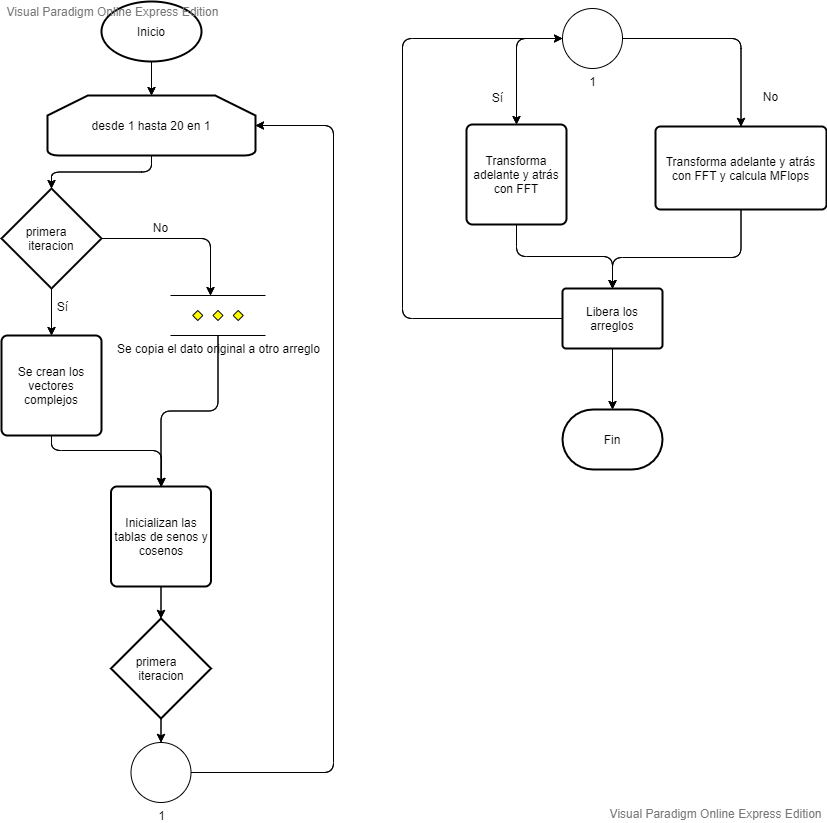
\includegraphics[scale=0.5]{Images/FFT_Paralelo.png}
    \caption{Diagrama de flujo de FFT en paralelo.}
\end{figure}

\clearpage
\section*{Pruebas}
Se realizaron pruebas entre la versión secuencial y la versión paralela  del algoritmo FFT a partir de la siguiente formula:\medskip
 
FFT ( FFT ( X(1:N) ) ) == N * X(1:N)\medskip

El lenguaje de programación implementado fue Open MP y el numero de núcleos fue de 4\medskip

Para N=1 Secuencial

\begin{figure}[h!]
    \centering
    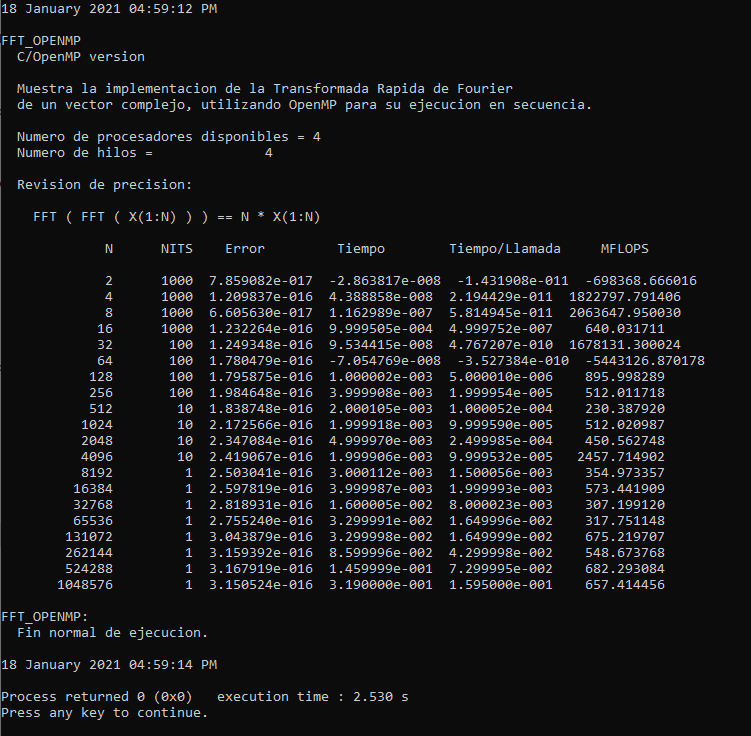
\includegraphics[scale=.8]{Images/FFT_Sec_1.png}
    \label{Secuencial 1.1}
\end{figure}

\clearpage

Para N=1 Paralelo\medskip

\begin{figure}[h!]
    \centering
    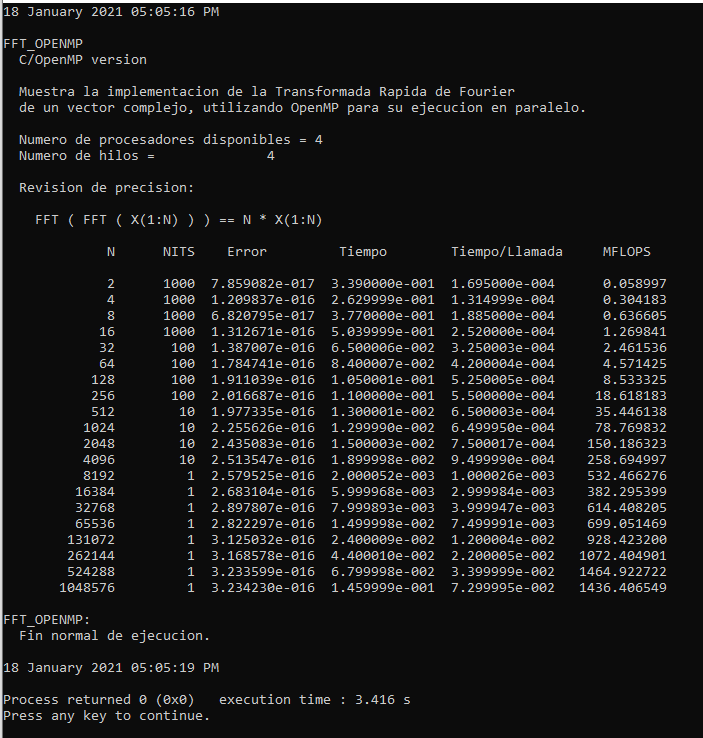
\includegraphics[scale=.8]{Images/FFT_Par_1.png}
    \label{Paralelo 1.1}
\end{figure}

\clearpage

Para N=10 Secuencial

\begin{figure}[h!]
    \centering
    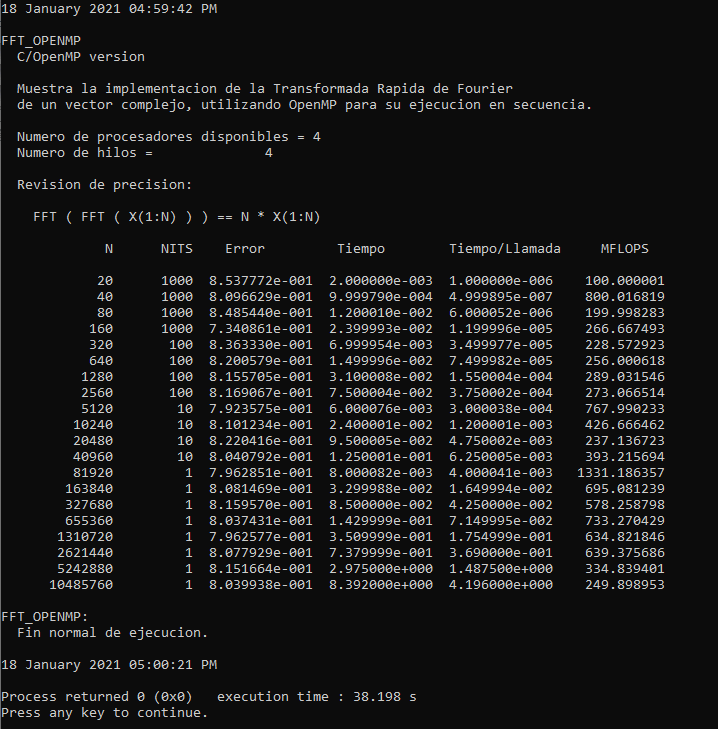
\includegraphics[scale=.8]{Images/FFT_Sec_10.png}
    \label{Secuencial 1.2}
\end{figure}

\clearpage

Para N=10 Paralelo\medskip

\begin{figure}[h!]
    \centering
    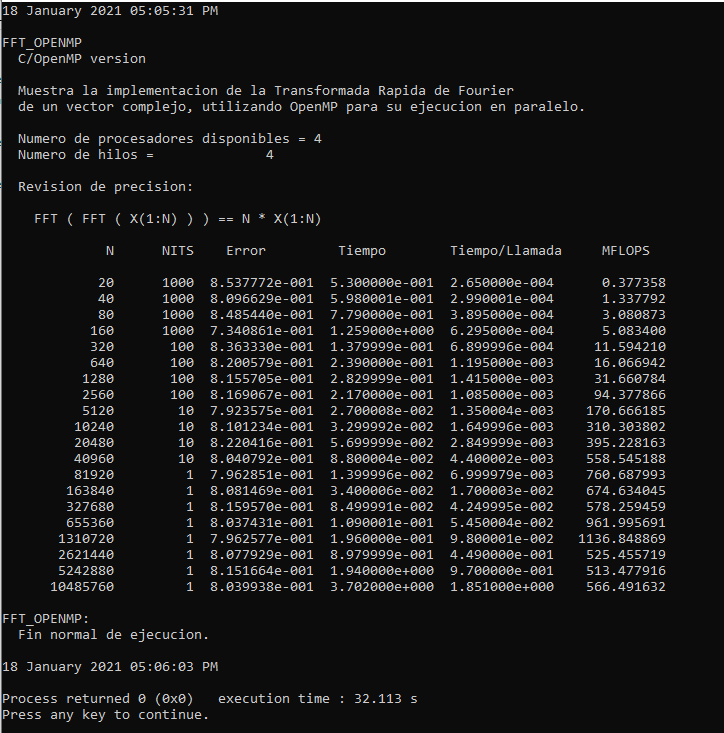
\includegraphics[scale=.8]{Images/FFT_Par_10.png}
    \label{Paralelo 1.2}
\end{figure}

\clearpage

Para N=50 Secuencial

\begin{figure}[h!]
    \centering
    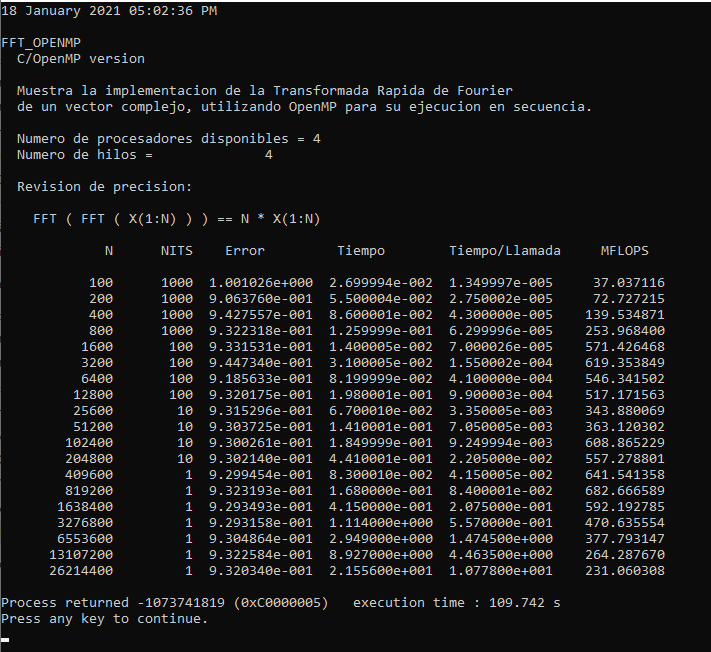
\includegraphics[scale=.8]{Images/FFT_Sec_50.png}
    \label{Secuencial 1.3}
\end{figure}

\clearpage

Para N=50 Paralelo\medskip

\begin{figure}[h!]
    \centering
    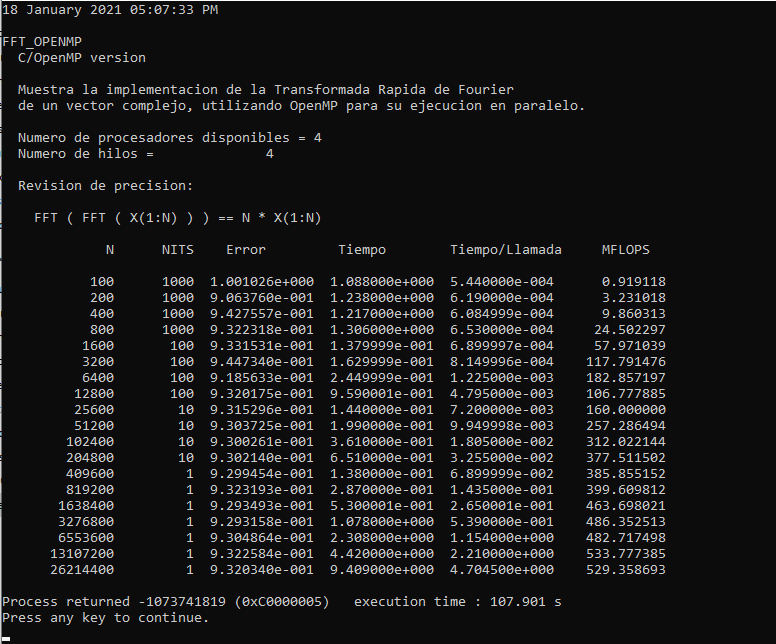
\includegraphics[scale=.8]{Images/FFT_Par_50.png}
    \label{Paralelo 1.3}
\end{figure}


\clearpage
Para N=100 Secuencial

\begin{figure}[h!]
    \centering
    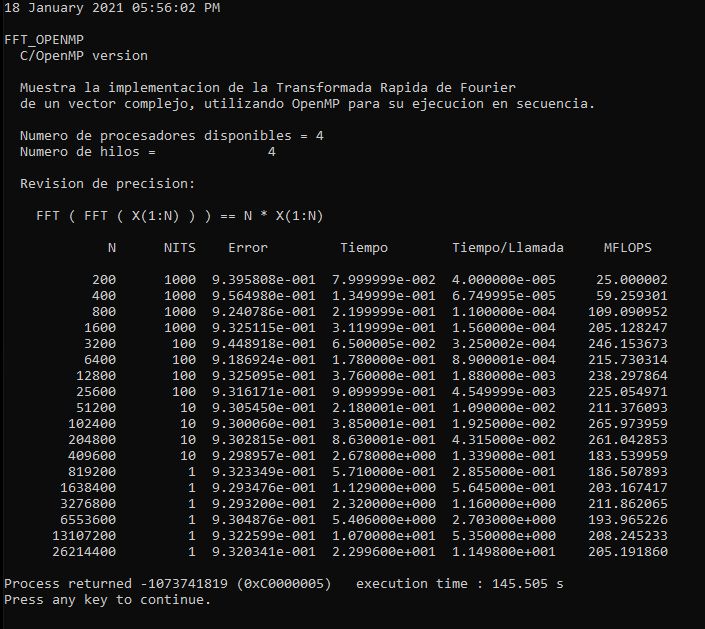
\includegraphics[scale=.8]{Images/FFT_Sec_100.png}
    \label{Secuencial 1.4}
\end{figure}

\clearpage

Para N=100 Paralelo\medskip

\begin{figure}[h!]
    \centering
    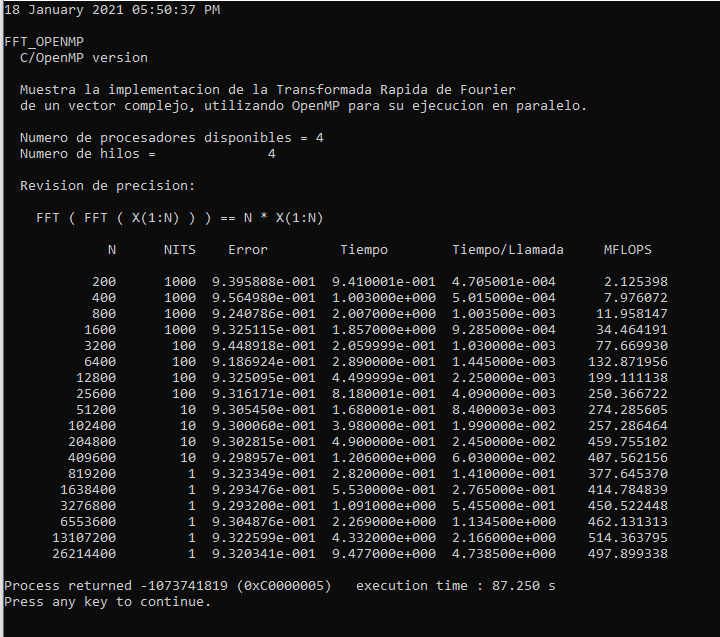
\includegraphics[scale=.8]{Images/FFT_Par_100.png}
    \label{Paralelo 1.4}
\end{figure}

\clearpage
Para N=200 Secuencial

\begin{figure}[h!]
    \centering
    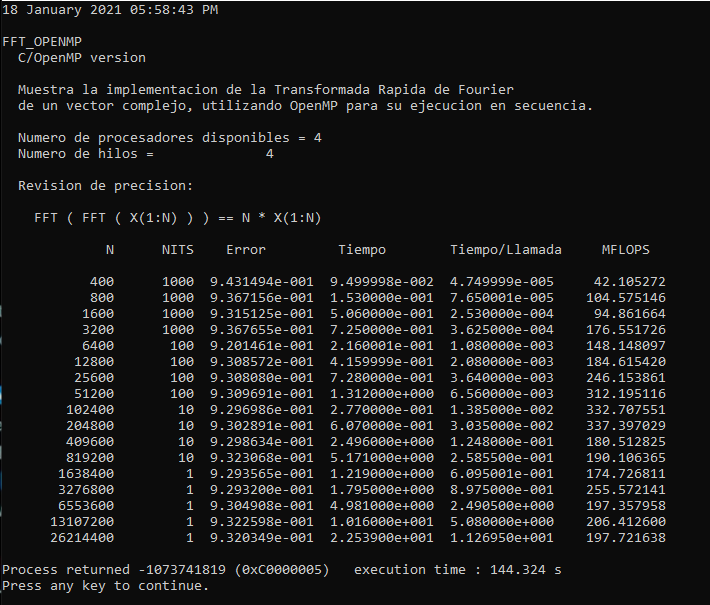
\includegraphics[scale=.8]{Images/FFT_Sec_200.png}
    \label{Secuencial 1.5}
\end{figure}

\clearpage
Para N=200 Paralelo\medskip

\begin{figure}[h!]
    \centering
    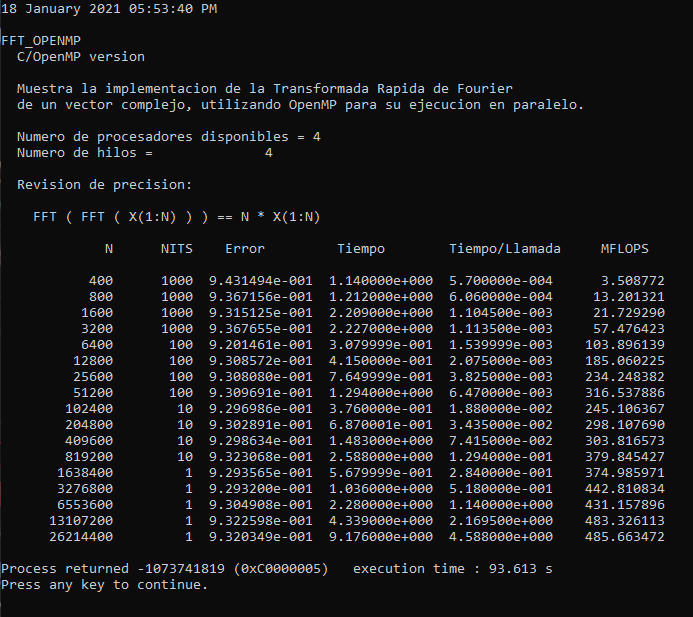
\includegraphics[scale=.8]{Images/FFT_Par_200.png}
    \label{Paralelo 1.5}
\end{figure}

\clearpage


\begin{figure}[h!]
    \centering
    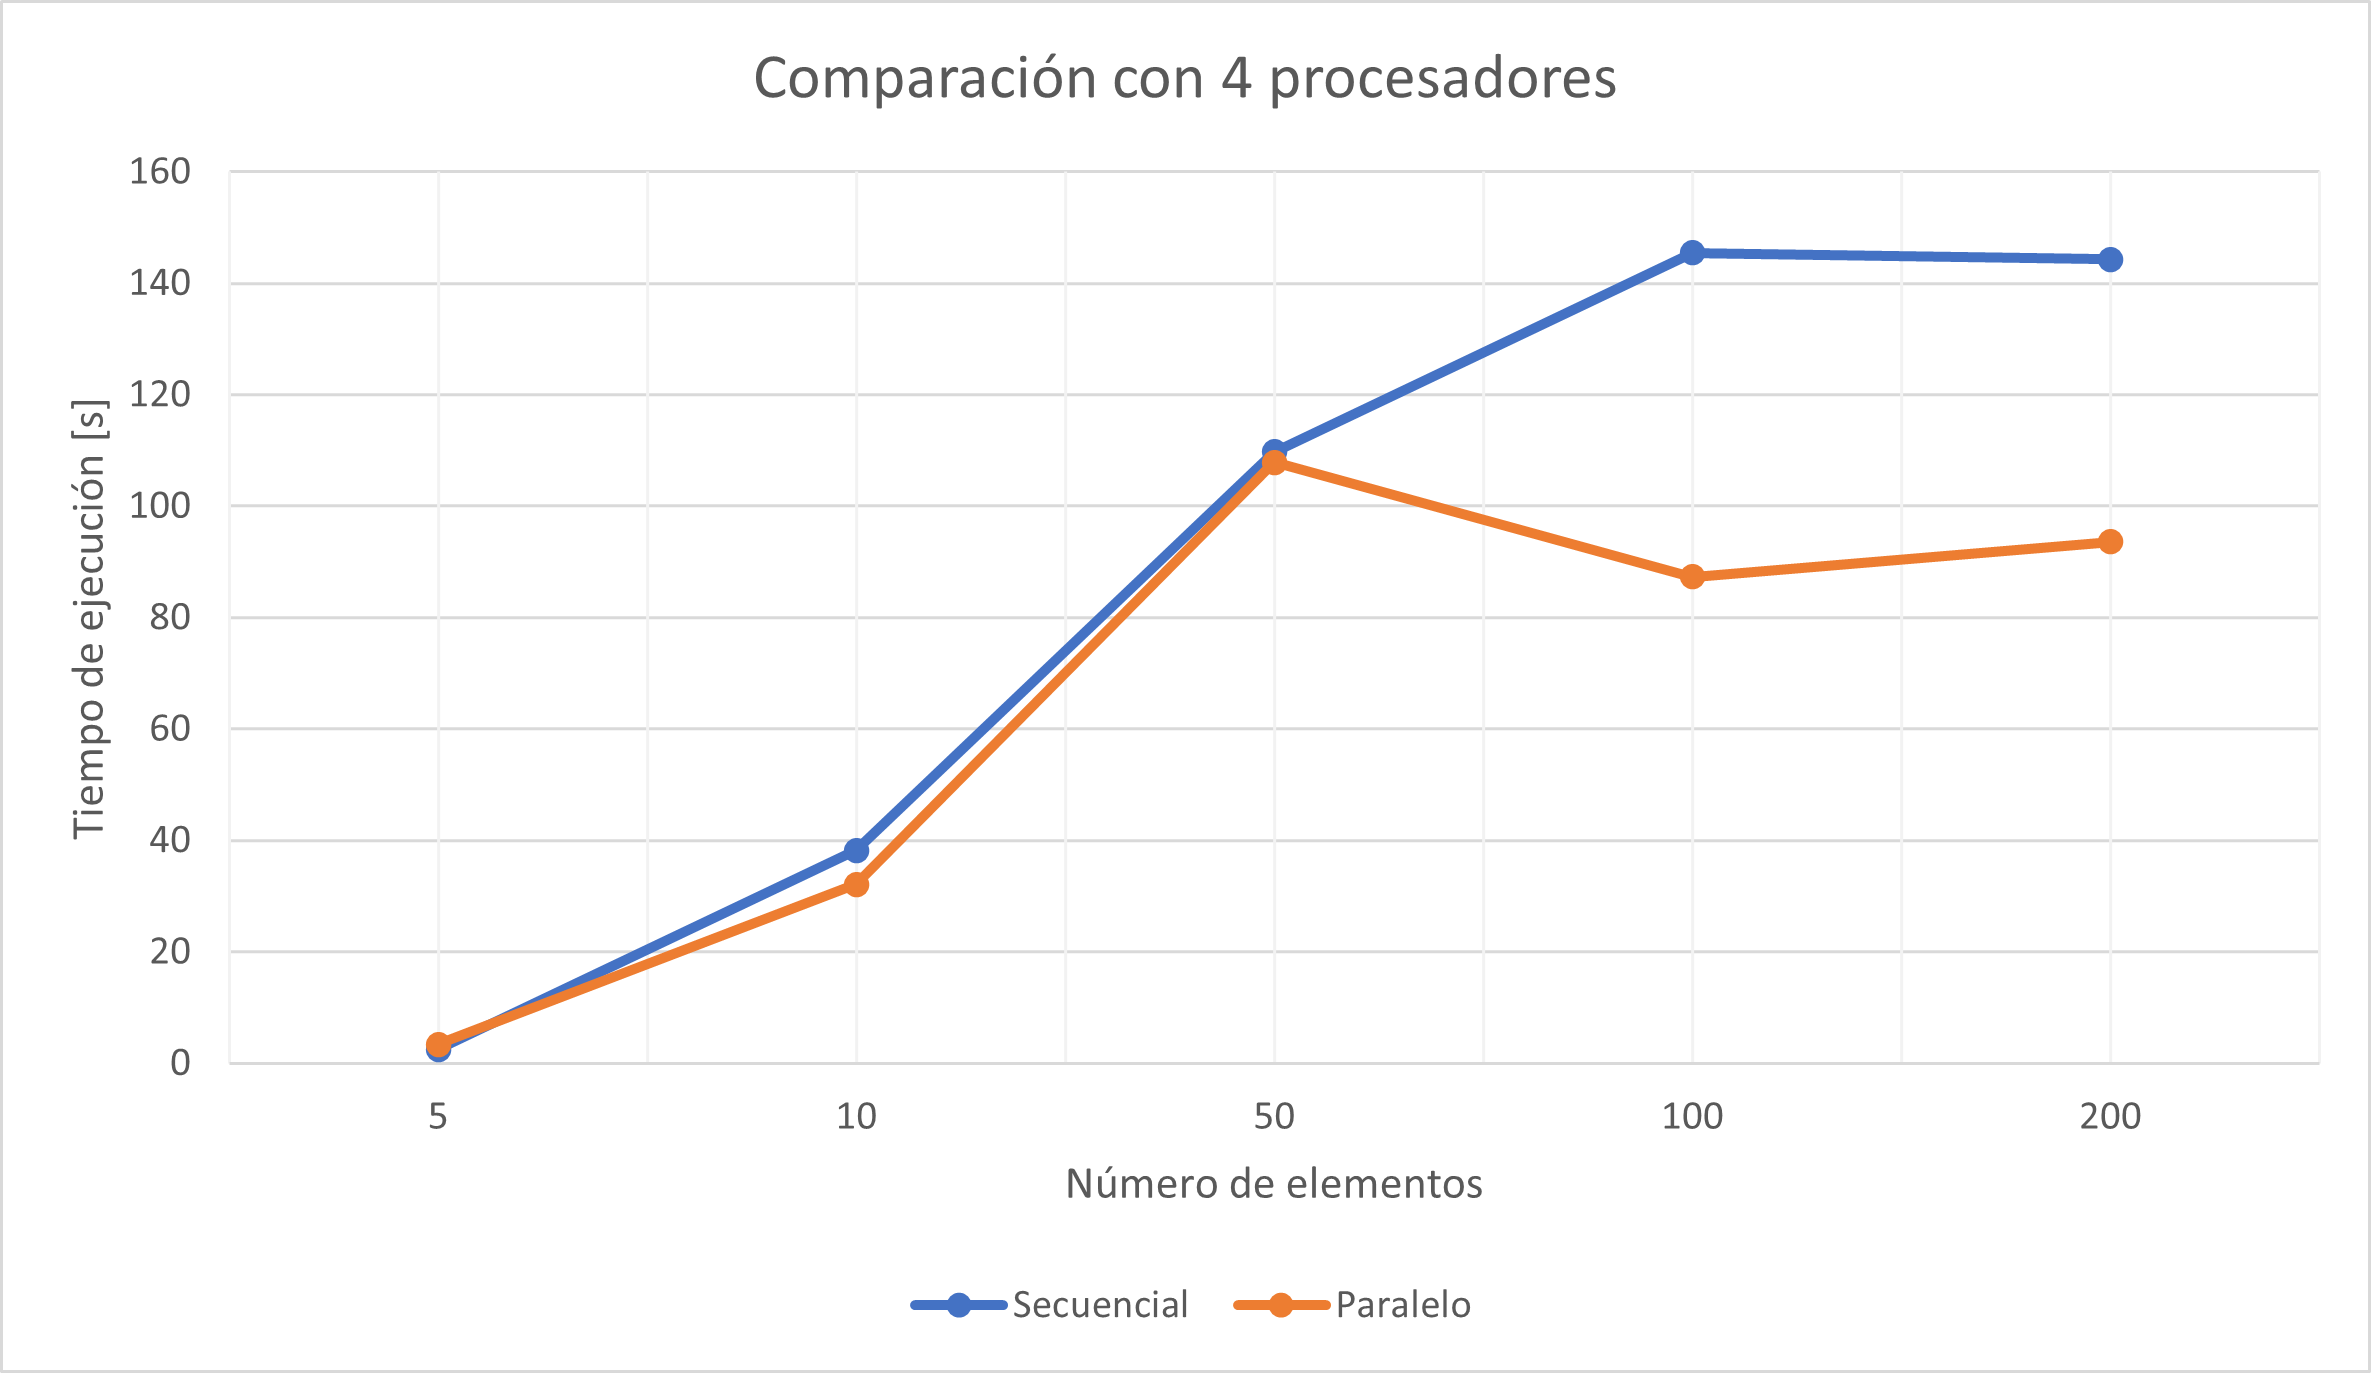
\includegraphics[scale=0.9]{Images/4_Procesadores.png}
    \caption{Gráfico comparativo entre el algoritmo secuencial y el algoritmo paralelo.}
\end{figure}

\clearpage
Para N=200 Secuencial 8 núcleos\medskip

\begin{figure}[h!]
    \centering
    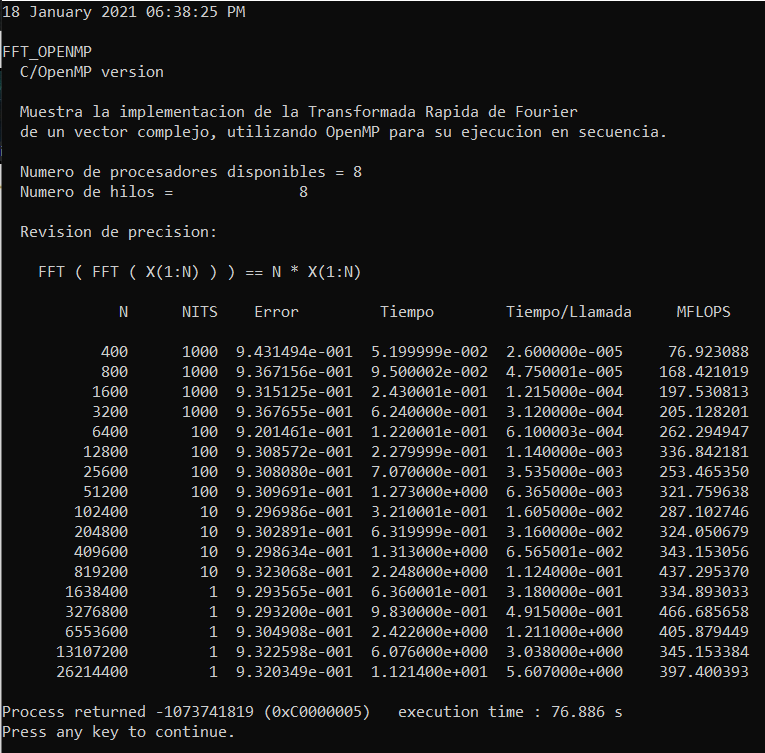
\includegraphics[scale=.8]{Images/FFT_Sec_200_8n.png}
    \label{Secuencial 1.6}
\end{figure}

\clearpage

Para N=200 Paralelo 8 núcleos\medskip

\begin{figure}[h!]
    \centering
    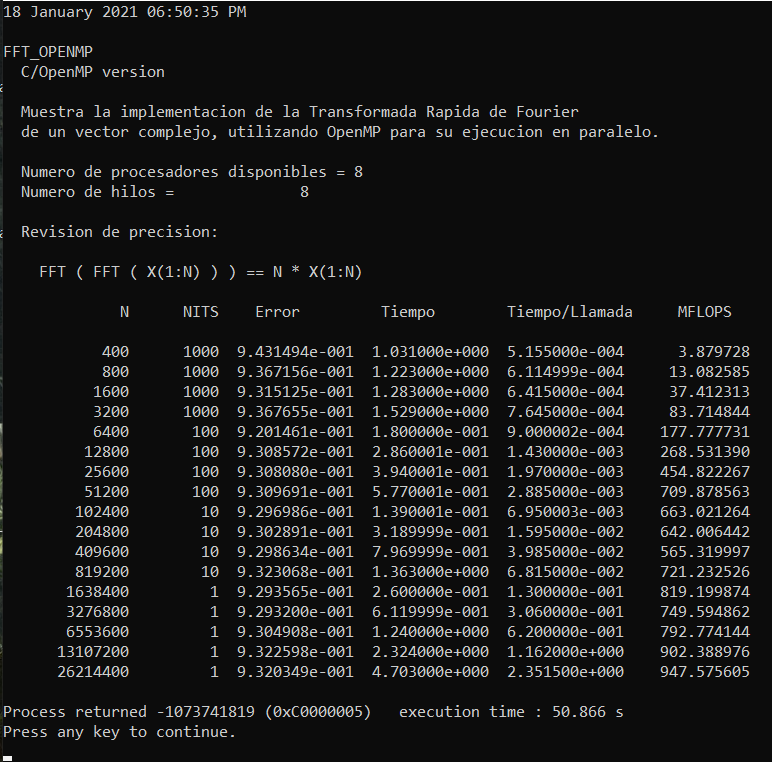
\includegraphics[scale=.8]{Images/FFT_Par_200_8n.png}
    \label{Paralelo 1.6}
\end{figure}

\clearpage
\section*{Conclusiones}
\noindent El algoritmo paralelo para la computación de la Transformada de Fourier, mejor conocido como Fast Fourier Transform (\textbf{FFT}) es uno de los algoritmos más utilizados y más importantes de los últimos tiempos. Quizá puede ser uno de los algoritmos más importantes en la historia debido a su gran rango de aplicaciones y a la relevancia que éstas tienen. De forma sencilla lo que el algoritmo hace es transformar las medidas experimentales de una onda electromagnética en una función analítica de frecuencia. Esto permite poder filtrar las señales, pero también conocer más información sobre ella. Algunos de sus usos con mayor repercusión son el internet, el GPS y la radio (nada más).\medskip

Es por esto que el poder realizar un algoritmo lo más eficiente posible en términos de computación fue esencial. Y así se llegó al FFT paralelo, con muchas implementaciones históricas y muchas investigaciones sobre como mejorarlo. Pero antes de poder analizar todo el aspecto del paradigma paralelo, primero se debe entender el algoritmo y esto resultó ser más complicado de lo que inicialmente pensamos.\medskip

En términos de los objetivos del proyecto, estos fueron cumplidos satisfactoriamente tanto en los generales como en los particulares. Durante el desarrollo del proyecto se afianzaron la gran mayoría de los conceptos vistos en la clase de teoría. Se reviso el funcionamiento de los procesadores en paralelo par poder hacer una buena ejecución que nos diera datos para el análisis. Se determinó el algoritmo tanto secuencial como paralelo de la transformada de Fourier, su tipo de paralelismo (de datos), topología de red (topología de red de mariposa), forma de comunicación (memoria compartida), granularidad (fina, mucha comunicación) y las diferentes métricas de desempeño con su análisis correspondiente. Con respecto a los objetivos particulares consideramos que sí se logró un gran entendimiento del algoritmo (tanto la parte lógica como matemática). Esto nos permitió dar una explicación clara del algoritmo y su paralelización como se puede apreciar en el video.\medskip

Finalmente el algoritmo FFT fue muy interesante de investigar y ver todas las aplicaciones que tiene en el mundo real y en nuestras vidas. Y el entender que de una forma paralela podemos mejorar su eficiencia nos dio un punto de vista más apreciativo sobre la programación paralela. En nuestro caso, la paralelización si representa una gran ventaja al secuencial. Por lo que sentimos aprendimos mucho de esta actividad del semestre.

\clearpage
\subsection*{David Calderón Jiménez}
Para mi este nuevo paradigma de programación es aparte de interesante muy útil pues nos abre las puertas a aplicaciones que difícilmente podríamos hacer en una programación secuencial.Desde mi punto de vista al nivel en el que estamos hilos me parece mas útil que propiamente la programación paralela pues los hilos nos permiten trabajar con programas sencillos los cuales necesitan realizar 2 o mas 
acciones al mismo tiempo y la programación paralela se aplica de mejor manera cuando se trabaja con enormes cantidades de información las cuales a nuestro nivel muy pocas veces hemos visto.

Por el momento me quedare con esta primera aproximación a la programación paralela pero a su vez se que es un tema que tiene muchas aplicaciones y un campo de investigación muy amplio por lo que en un futuro yo desearía profundizarlo mas.

\subsection*{Humberto Ignacio Hernández Olvera}
Este nuevo paradigma de programación, definitivamente es algo que se me complica entender, quizás la lógica en las líneas de los códigos es algo que puedo seguir, ya que al final de cuentas, sigue siendo código muy similar a lo que estuvimos trabajando previamente, el hecho de poder identificar en donde se tiene que hacer la paralelización es lo que me causa ruido, al igual que encontrar la aplicación del paradigma, es algo que tendría que reforzar para poder llegar a un entendimiento adecuado del paradigma.\medskip

En cuanto al algoritmo que desarrollamos, veo que la Transformada de Fourier tiene una buena aplicación en el campo de la física y la ingeniería. Con este primer acercamiento, y teniendo una idea de cómo es que se puede programar, creo que ayudará bastante para los siguientes retos a los que nos enfrentemos en la carrera más adelante, ya que no llegaremos en blanco.\medskip

\subsection*{Iñaky Ordiales Caballero}
El proyecto en general me gustó y me pareció algo desafiante. Si bien la implementación en código no es difícil de seguir, el entender a un buen nivel el algoritmo secuencial para luego ir al paralelo requiere de una revisión de las matemáticas detrás de él. Esto hizo que nos tardáramos más tiempo en la parte escrita, ya que sentimos que no hacía sentido presentar el algoritmo sin el contexto anterior adecuado. Por lo que las primeras páginas sirven de introducción al algoritmo, tanto en el ámbito matemático como en el de la computación paralela. Finalmente el algoritmo FFT fue muy interesante de investigar y ver todas las aplicaciones que tiene en el mundo real y en nuestras vidas. Y el entender que de una forma paralela podemos mejorar su eficiencia nos dio un punto de vista más apreciativo sobre la programación paralela. Por lo que sentí que aprendimos mucho de esta actividad del semestre.

\clearpage

\subsection*{Autoevaluación}
El momento de mirar atrás y auto evaluar un proyecto que realizamos siempre es un proceso interesante. Si bien mientras lo elaboramos nos damos cuenta de nuestras dificultades y fortalezas de lo que se va haciendo y escribiendo en el reporte. No es hasta este punto donde ya todo quedó finalizado, donde se hicieron varias lecturas de prueba y finalmente se decidió no modificar nada más, que realmente podemos evaluar la calidad y claridad de la información y del trabajo en general.\medskip

Al momento de iniciar con la elaboración del proyecto de investigación buscamos algunas opciones de algoritmos y enviamos nuestra propuesta. El que se decidió que hiciéramos fue el algoritmo para computar la Transformada de Fourier. Y a pesar de haber leído un poco al respecto antes de enviarlo como posible opción, realmente no investigamos a profundidad hasta estar seguros que fue el elegido. Para el momento en que nos adentramos más en el algoritmo creo que nos dimos cuenta que para entenderlo, tendríamos que entender las matemáticas detrás de él. Y a pesar de no ser las más complicadas, sí representaron un desafío. Sin embargo pudimos leer muchos recursos y ver varios videos en internet para comprenderla por completo. A partir de que comprendimos el algoritmo, pudimos empezar a realizar todo el análisis de la paralelización junto con las pruebas que conllevan.\medskip

Para no seguirnos alargando mucho, consideramos que todo el proceso desde el cómo y de dónde sale el algoritmo secuencial, hasta la parte de paralelizarlo, ver la topología, comunicación y granularidad que tiene está claramente explicado en este documento. Además el video deja claro lo más importante sobre el algoritmo paralelo, que era lo principal del proyecto. Por lo que consideramos que el trabajo entregado en todas sus diferentes partes es de buena calidad y con el que nos sentimos satisfechos. De poder cambiar algo, probablemente nos hubiera gustado hacer muchas más pruebas para poder tener más información analizable sobre el paralelismo del algoritmo. Pero debido a los núcleos de nuestras compus no lo pudimos hacer. Por lo demás sentimos el trabajo es muy bueno.\medskip

Poner un número para representar tu propio trabajo siempre es difícil. Muchas veces podemos terminar no siendo objetivos o por el contrario sobrecompensar y ser muy estrictos. Haciendo nuestro mejor esfuerzo para evitar esto, pensamos que el trabajo merece un \textbf{9.5} ya que si bien no es perfecto, es muy bueno y cumple con los requisitos.

\nocite{*}
\printbibliography[title={Fuentes de información}]

\end{document}
